\chapter{Einführung}

\label{cha_cryptographic_techniques}

In diesem Kapitel soll ein kurzer Überblick über die im Laufe der Arbeit relevanten kryptographischen Verfahren gegeben werden sowie die verwendete Notation vorgestellt werden.\todo{um Schutzziele erweitern}

\section{Kryptographische Verfahren}

\subsection{Symmetrische Kryptographie}

Symmetrische Kryptographie beschreibt Verfahren, bei denen für Ver- und Entschlüsselung der gleiche (oder ein aus dem anderen Schlüssel leicht berechenbarer) Schlüssel verwendet wird \cite{Schneier2006}. Vor einer Kommunikation müssen beide Kommunikationspartner im Besitz dieses Schlüssels sein. Die Sicherheit der Verfahren liegt in der Geheimhaltung des Schlüssels,  der über einen sicheren Kanal ausgetauscht worden sein muss.
Es gilt:
\[E_K(M)=C\] 
\[D_K(C)=M\] 
Hierbei steht \(M\) für die Nachricht, \(K\) für den Schlüssel, der verwendet wird, \(C\) für den Chiffretext und \(E\) für die Ver- bzw. \(D\) für die  Entschlüsselung. Der Vorgang der symmetrischen Ver- und Entschlüsselung wird in Abbildung \ref{fig_symmetric_encryption} dargestellt.

\begin{figure}
	\centering
	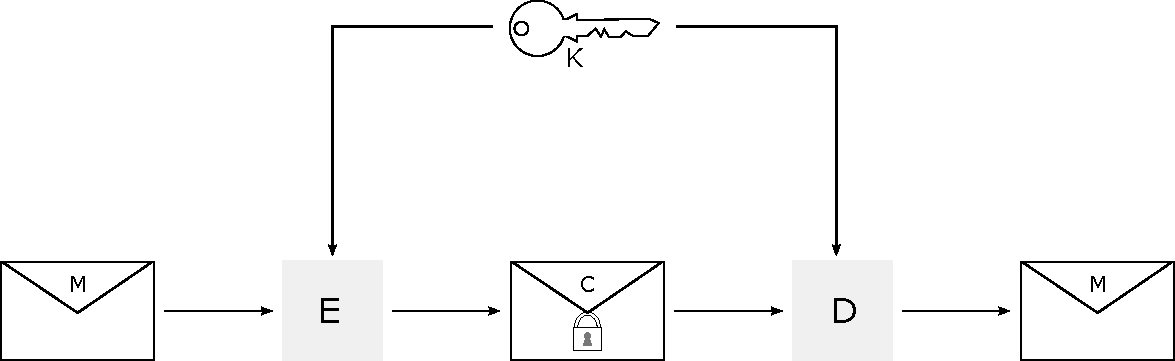
\includegraphics[width=15cm]{Diagrams/SymmetricEncryption.pdf} %
	\caption{Symmetrische Kryptographie}
	\label{fig_symmetric_encryption}
\end{figure}

Symmetrischen Chiffren lassen sich in Strom- und Blockchiffren unterteilen.

\subsubsection{Stromchiffren}

Stromchiffren sind symmetrische Verschlüsselungsalgorithmen, die Klartexte bitweise zu Chiffretexten konvertieren \cite{Schneier2006}. Die einfachste Möglichkeit ist die XOR-Verknüpfung der Klartextbits mit einem schlüsselabhängig generierten Bitstrom (Schlüsselstrom). Durch erneute XOR-Verknüpfung mit demselben Schlüsselstrom auf der Empfängerseite lässt sich der Klartext zurückerhalten. Ein Beispiel für eine heute verwendete Stromchiffre ist RC4.

\subsubsection{Blockchiffren}

\label{sec_block_cipher}

Bei Blockchiffren handelt es sich um symmetrische Verschlüsselungsalgorithmen, die Nachrichten in Blöcken fester Größe verschlüsseln \cite{Schneier2006}. Beispiele für heute verwendete Blockchiffren sind AES oder Twofish.

Da eine Blockchiffre immer nur einen Block verschlüsseln kann, muss festgelegt werden, wie mit mehreren Blöcken verfahren werden soll. Die Beschreibung eines solchen Verfahrens wird Betriebsmodus genannt.

Der einfachste Modus ist der ECB-Modus (Electronic Codebook). In diesem Modus wird jeder Block einzeln und unabhängig von anderen Blöcken verschlüsselt. Dieser Modus ist als unsicher zu betrachten, da die Verschlüsselung gleicher Klartextblöcke mit gleichem Schlüssel immer zu dem gleichen Chiffretextblock führt und ein Angreifer außerdem nach Belieben einzelne Blöcke entfernen, hinzufügen oder austauschen kann, ohne dass dies zwingend bemerkt wird.

Ein weiterer, häufig verwendeter Modus ist CBC (Cipher Block Chaining). Hierbei erfolgt eine XOR-Verknüpfung des zuletzt erhaltenen Chiffretextblocks mit dem nächsten Klartextblock vor seiner Verschlüsselung. Zusätzlich wird für den ersten Klartextblock ein zusätzlicher, zufällig gewählter Block, der sogenannte Initialisierungsvektor (IV), benötigt \cite{Schneier2006}.

Einen Sonderfall stellen die AEAD-Chiffren (Authenticated Encryption with Associated Data) dar. Hierbei handelt es sich um Betriebsmodi, die ohne zusätzlichen Message Authentication Code (siehe Abschnitt \ref{sec_mac}) Authentizität und Integrität bereitstellen. Beispiele für solche Modi sind CCM (Counter with CBC-MAC) oder GCM (Galois/Counter Mode). 

\subsection{Asymmetrische Kryptographie}

Asymmetrische Kryptographie (oftmals auch Public-Key-Kryptographie) beschreibt Verfahren, bei denen für Ver- und Entschlüsselung verschiedene Schlüssel verwendet werden \cite{Schneier2006}. Die Sicherheit der Verfahren beruht darauf, dass der öffentliche Schlüssel sich nicht mit vertretbarem Aufwand aus dem geheimen Schlüssel berechnen lässt. Daher kann ein Empfänger seinen öffentlichen Schlüssel bekanntgeben. Nachrichten, die mit diesem Schlüssel verschlüsselt werden, kann ein Angreifer dennoch nicht lesen, solange er nicht im Besitz des geheimen Schlüssels ist. Es gilt: 
\[E_{K_{\text{public}}}(M)=C\] 
\[D_{K_{\text{private}}}(C)=M\] 
Hierbei steht \(K_{\text{public}}\) für den öffentlichen und \(K_{\text{private}}\) für den geheimen Schlüssel des Empfängers. Der Vorgang der asymmetrischen Ver- und Entschlüsselung ist in Abbildung \ref{fig_asymmetric_encryption} dargestellt.

\begin{figure}
	\centering
	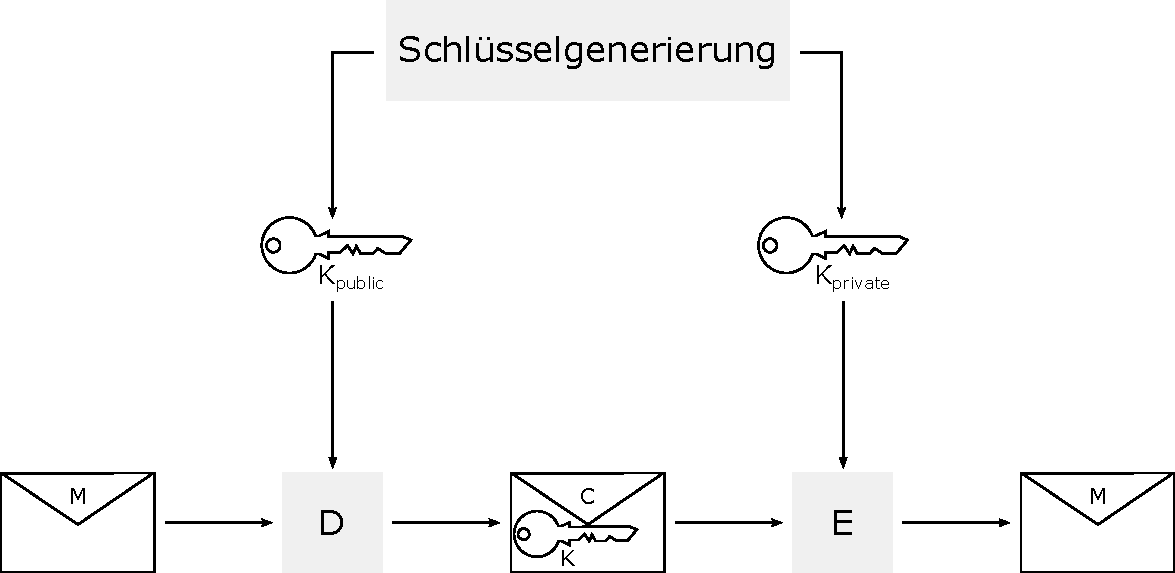
\includegraphics[width=15cm]{Diagrams/AsymmetricEncryption.pdf} %
	\caption{Asymmetrische Kryptographie}
	\label{fig_asymmetric_encryption}
\end{figure}

Weiterhin können asymmetrische Verfahren auch zur Signierung von Nachrichten genutzt werden, indem der Verfasser die Nachricht (bzw. aus Effizienzgründen in der Praxis einen Hashwert der Nachricht) mit seinem geheimen Schlüssel verschlüsselt und an die Nachricht anhängt. Dieser Vorgang wird signieren genannt. Empfänger können nun durch Entschlüsselung mit dem öffentlichen Schlüssel und Vergleich mit der empfangenen Nachricht (bzw. ihrem Hashwert) die Signatur überprüfen. 

Durch asymmetrische Kryptographie lässt sich das bei symmetrischen Algorithmen bestehende Problem des Schlüsselaustauschs durch Veröffentlichung des öffentlichen Schlüssels leicht lösen. Das Problem, das hierbei besteht, ist es jedoch, die Identität des Besitzers eines öffentlichen Schlüssels sicherzustellen.

Ein Beispiel für einen asymmetrischen Algorithmus ist das RSA-Verfahren \cite{Schneier2006}.

\subsection{Diffie-Hellmann-Verfahren}

\label{sec_diffie_hellman}

Das Diffie-Hellmann-Verfahren (DH-Verfahren) ist ebenfalls ein auf geheimen und öffentlichen Schlüsseln basierendes Verfahren, das jedoch nicht der Ver- bzw. Entschlüsselung, sondern lediglich der Schlüsselvereinbarung dient. Es ermöglicht zwei Kommunikationspartnern, einen symmetrischen Schlüssel zu erzeugen, ohne dass dieser direkt gesendet werden muss \cite{dh76}. 

Die Partner \(A\) und \(B\) einigen sich auf eine Gruppe primer Ordnung \(p\) und eine Zahl \(g\), die die Gruppe erzeugt. Zusätzlich wählt jeder Partner eine große, zufällige Zahl \(X\) als privaten Schlüssel. Dann berechnet jeder Partner seinen öffentlichen Schlüssel \(Y\) folgendermaßen:
\begin{align*}
&Y_A = g^{X_A} \mod{p} \text{ \hspace{0.5cm} bzw.}\\
&Y_B = g^{X_B} \mod{p}
\end{align*}
Diese Werte werden nun an den anderen Partner gesendet und der gemeinsame Schlüssel \(K\) kann berechnet werden:
\begin{align*}
&K = Y_B^{X_A} \mod{p} = (g^{X_B})^{X_A }\mod{p} = g^{X_A X_B}\mod{p} \text{ \hspace{0.5cm} bzw.}\\
&K = Y_A^{X_B} \mod{p} = (g^{X_A})^{X_B }\mod{p} = g^{X_A X_B}\mod{p} 
\end{align*}
Ein Angreifer, der lediglich im Besitz von \(Y_A\) und \(Y_B\) ist, kann den Schlüssel nur schwer berechnen. 

\subsection{Hashfunktion}

Eine Hashfunktion ist eine Funktion, die eine Eingabe variabler Länge auf eine Ausgabe fester Länge(den Hashwert) abbildet \cite{Schneier2006}.

In der Kryptographie werden insbesondere Einweg-Hashfunktionen eingesetzt. Bei dieser Art von Hashfunktionen ist es leicht, aus einer Eingabe den Hashwert zu berechnen, jedoch sehr schwer, zu einem gegebenen Hashwert eine Eingabe zu finden, die auf diesen Wert abgebildet wird \cite{Schneier2006}. \\Ein Beispiel für heute verwendete Hashfunktionen ist SHA256.

\subsection{Message Authentication Code}

\label{sec_mac}

Ein Message Authentication Code (MAC) ist ein Verfahren, das dazu dient, die Authentizität und die Integrität einer Nachricht sicherzustellen. Dazu wird vom Sender aus einem geheimen Schlüssel \(K\) und der Nachricht \(M\) eine Art Prüfsumme generiert und zusammen mit der Nachricht versendet. Der Empfänger kann den MAC überprüfen, wenn er im Besitz des gleichen geheimen Schlüssels ist, und so sicher sein, dass die Nachricht nicht verändert wurde. Ein Beispiel für einen solchen MAC ist der auch in TLS verwendete HMAC \cite{Schneier2006, ferguson10}.

\section{Schutzziele}
\todo{Schreib es auf! Werden schon in 2.1.5 (MAC) genutzt.}

\subsection{Vertraulichkeit}

\subsection{Integrität}

\subsection{Verfügbarkeit}

\section{Verwendete Notationen}

In den folgenden Kapiteln werden die unten stehenden Notationen verwendet. Aus anderen Veröffentlichungen entnommene Passagen wurden teilweise geringfügig angepasst, um diesen Notationen zu folgen.

\(|B|\) steht für die Länge einer Zeichenkette B.

\(A \oplus B\) entspricht der bitweisen XOR-Verknüpfung zweier Zeichenketten A und B.

\(A + B\) steht für die Konkatenation zweier Zeichenketten A und B.

\(0x\dots\) entspricht einer Zahl im hexadezimalen System.

